\documentclass[tikz,border=8pt]{standalone}
\usetikzlibrary{arrows.meta,positioning}
\begin{document}
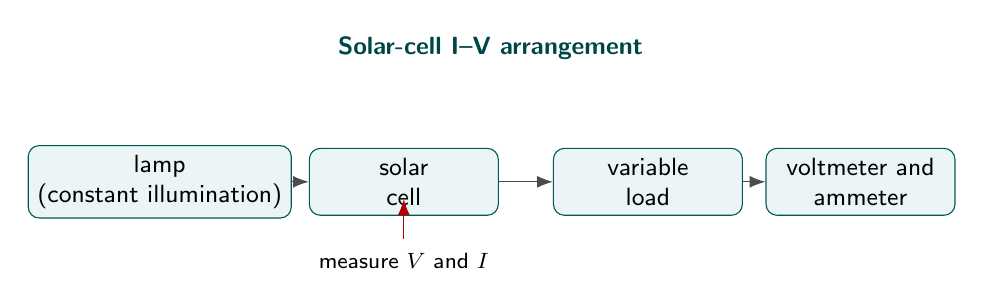
\begin{tikzpicture}[box/.style={draw=teal!70!black,fill=teal!8,rounded corners,minimum width=2.4cm,minimum height=.85cm,align=center,font=\sffamily\small},a/.style={-{Latex[length=2mm]},draw=black!70}]
\node[font=\sffamily\bfseries\small,text=teal!55!black] at (0,1.7) {Solar-cell I--V arrangement};
\node[box] (lamp) at (-4.2,0) {lamp\\(constant illumination)};
\node[box] (cell) at (-1.1,0) {solar\\cell};
\node[box] (load) at (2.0,0) {variable\\load};
\node[box] (meters) at (4.7,0) {voltmeter and\\ammeter};
\draw[a] (lamp)--(cell); \draw[a] (cell)--(load); \draw[a] (load)--(meters);
\node[font=\sffamily\footnotesize] at (-1.1,-1.0) {measure $V$ and $I$};
\draw[-{Latex[length=2mm]},draw=red!70!black] (-1.1,-.72)--(-1.1,-.22);
\end{tikzpicture}
\end{document}
